\documentclass{article}
\usepackage[utf8]{inputenc}
\usepackage[margin=1in]{geometry}
\usepackage{pdfpages}
\usepackage{hyperref}

\title{Project Report: How does BERT answer questions?}
\author{Kevin Kässens, Enno Teßmer}
\date{Deep Learning 2021}

\begin{document}
	\maketitle
	\section{Introduction}
	In this report, we present the results we achieved while working on our Deep Learning project. For our self-written code and any other additional files, we created a GitHub repository that can be found at \url{https://github.com/UNF-B5S/dl-project}.
	
	\section{Reproduced}
	\subsection{Visualization}
	We reproduced the visualization results using the hidden\_state\_visualizer.py script from the explain-BERT-QA repository. We used the SQuAD and bAbI models from the VisBERT models and created the samples with the question, answer and context according to the examples in the paper.
	You can find our results in the figures below. In the last figure it is clearly visible that BERT was able to extract the correct answer to the question in both cases.
	
	To see the plot for each hidden layer of an example, check the subfolder corresponding to the example in ./badges/reproduced/visualization.
	
	\subsubsection{SQuAD example}
	
	\begin{tabular}{ l p{0.85\linewidth} }
		Question: & What is a common punishment in the UK and Ireland? \\
		Answer: & detention \\
		Context: & Currently detention is one of the most common punishments in schools in the United States, the UK, Ireland, Singapore and other countries. It requires the pupil to remain in school at a given time in the school day (such as lunch, recess or after school); or even to attend school on a non-school day, e.g. \"Saturday detention\" held at some schools. During detention, students normally have to sit in a classroom and do work, write lines or a punishment essay, or sit quietly. \\
	\end{tabular}
	
	\begin{center}
		\begin{tabular}{ c c }
			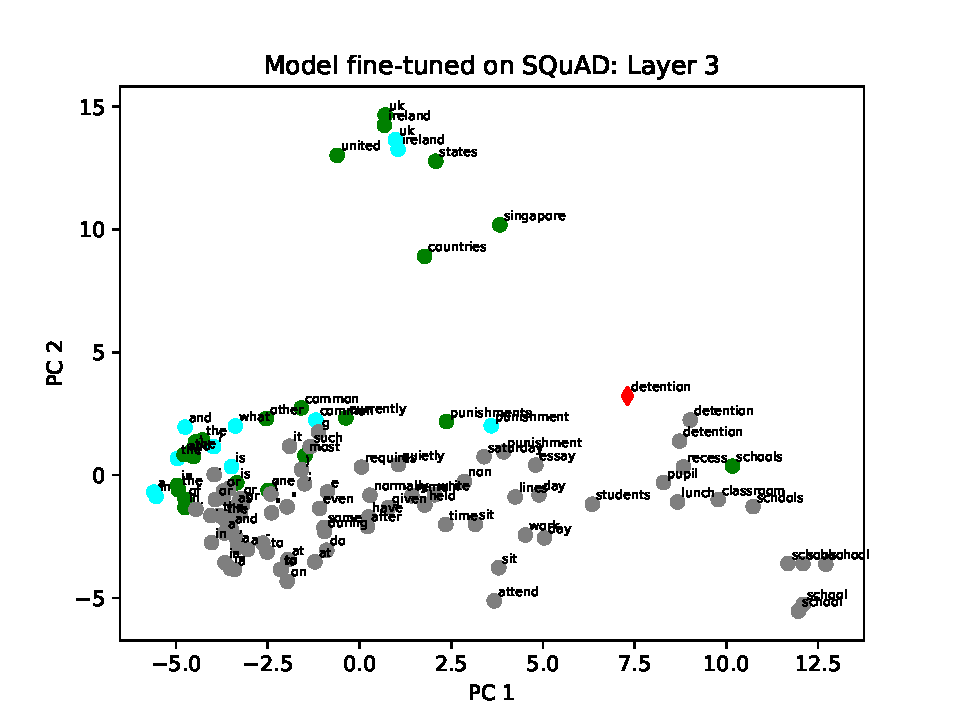
\includegraphics[scale=0.4]{../badges/reproduced/visualization/squad/model-fine-tuned-on-squad--layer-3.pdf} &
			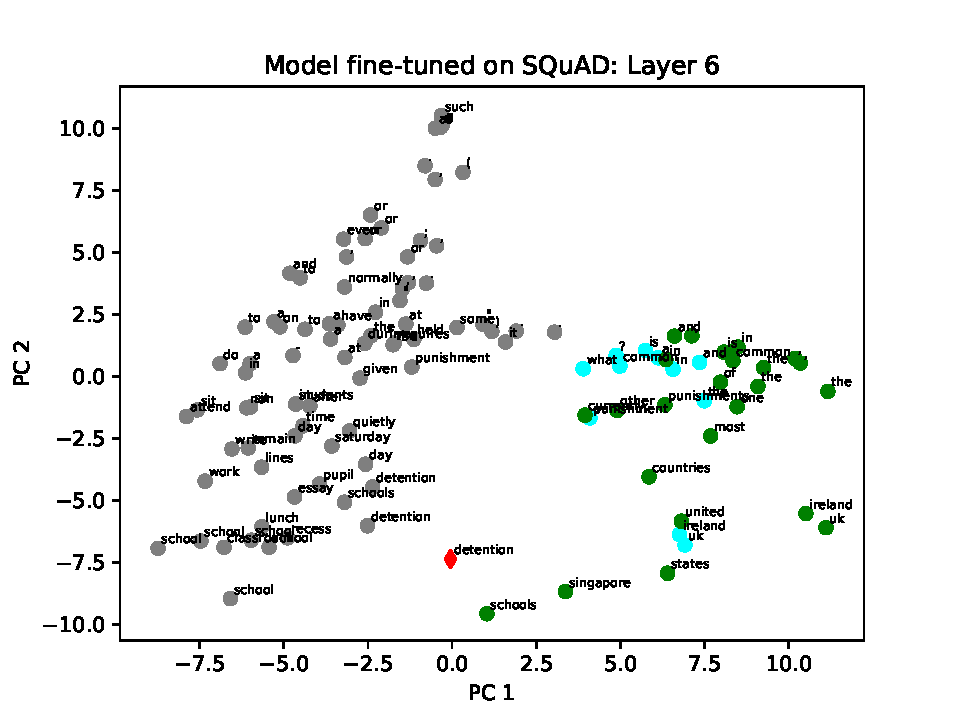
\includegraphics[scale=0.4]{../badges/reproduced/visualization/squad/model-fine-tuned-on-squad--layer-6.pdf}
		\end{tabular}
	\end{center}

	\begin{center}
		\begin{tabular}{ c c }
			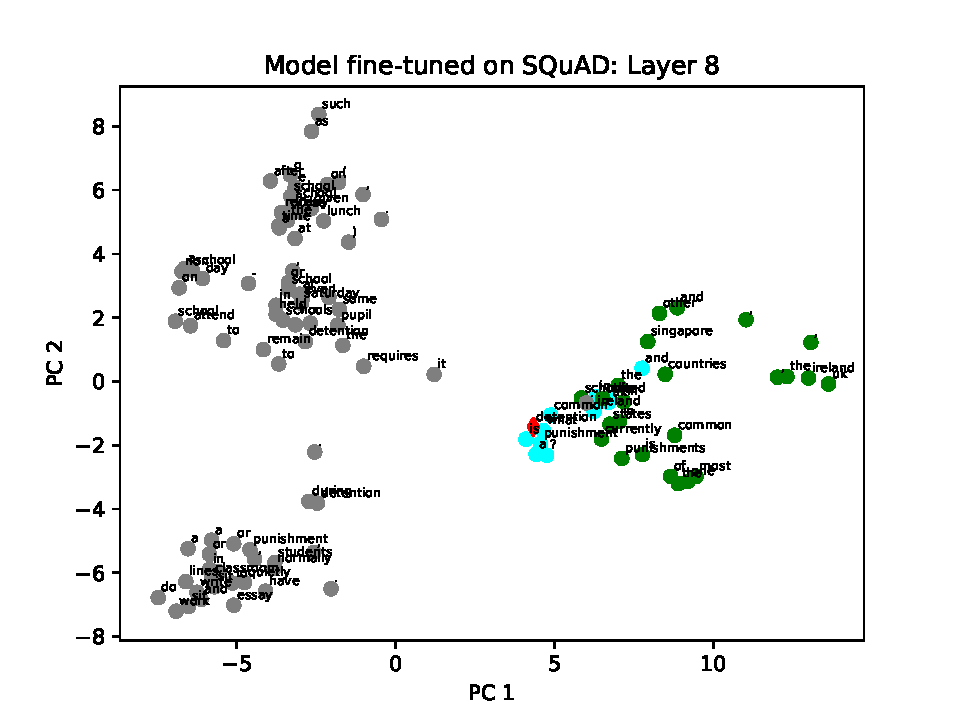
\includegraphics[scale=0.4]{../badges/reproduced/visualization/squad/model-fine-tuned-on-squad--layer-8.pdf} &
			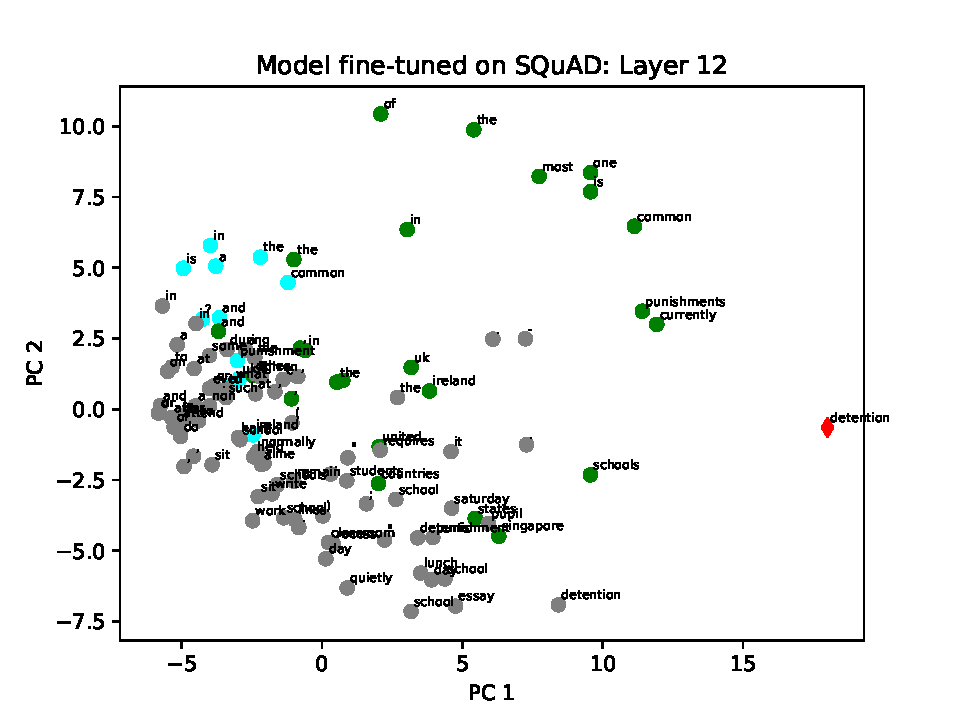
\includegraphics[scale=0.4]{../badges/reproduced/visualization/squad/model-fine-tuned-on-squad--layer-12.pdf}
		\end{tabular}
	\end{center}

	\subsubsection{bAbI example}

	\begin{tabular}{ l p{0.85\linewidth} }
		Question: & What is Emily afraid of? \\
		Answer: & cats \\
		Context: & Wolves are afraid of cats. 
		
		Sheep are afraid of wolves. 
		
		Mice are afraid of sheep. 
		
		Gertrude is a mouse. 
		
		Jessica is a mouse. 
		
		Emily is a wolf. 
		
		Cats are afraid of sheep. 
		
		Winona is a wolf. \\
	\end{tabular}
	
	\begin{center}
		\begin{tabular}{ c c }
			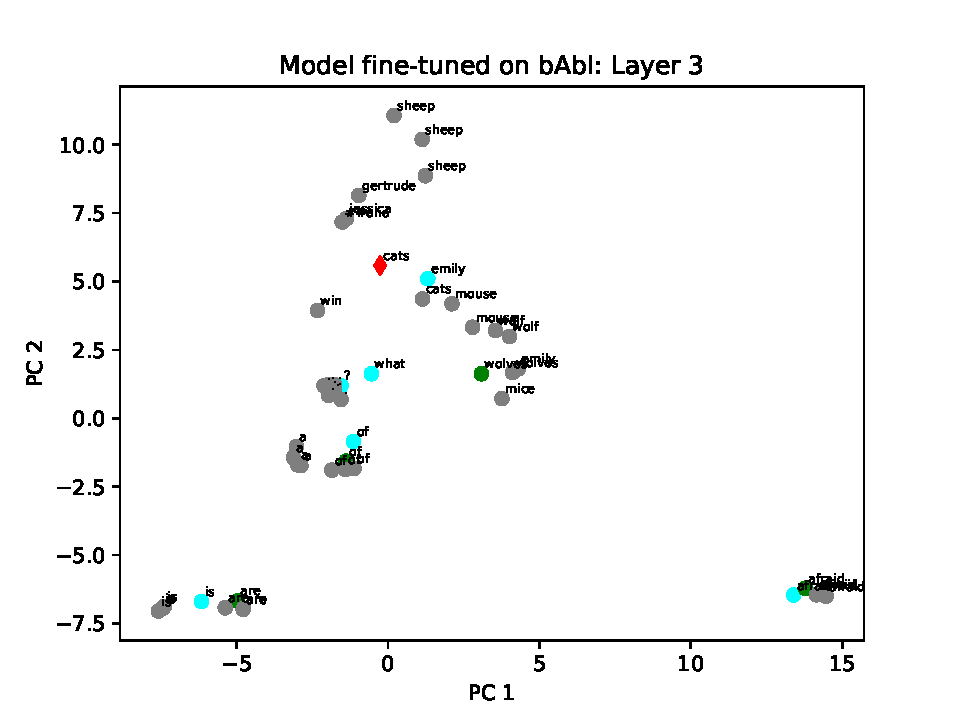
\includegraphics[scale=0.4]{../badges/reproduced/visualization/babi/model-fine-tuned-on-babi--layer-3.pdf} &
			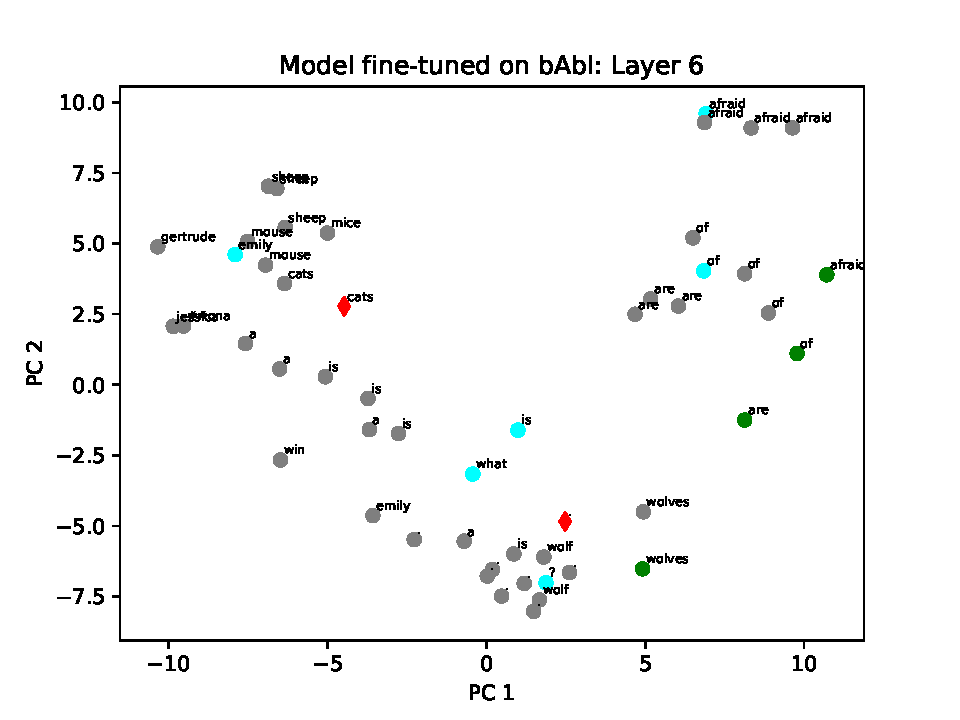
\includegraphics[scale=0.4]{../badges/reproduced/visualization/babi/model-fine-tuned-on-babi--layer-6.pdf} 
		\end{tabular}
	\end{center}

	\begin{center}
		\begin{tabular}{ c c }
			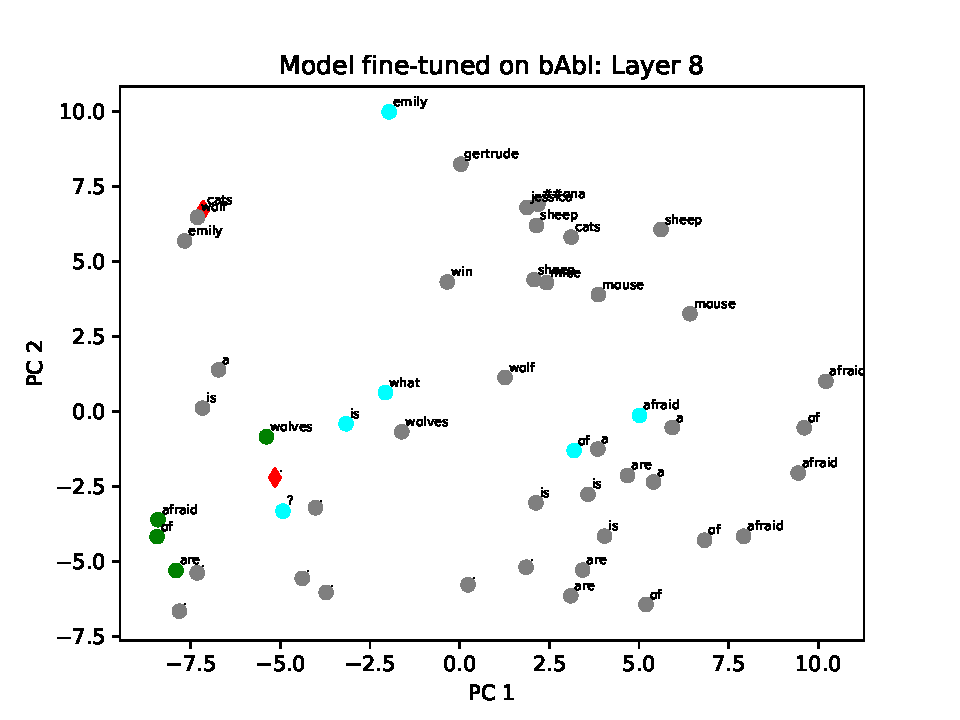
\includegraphics[scale=0.4]{../badges/reproduced/visualization/babi/model-fine-tuned-on-babi--layer-8.pdf} &
			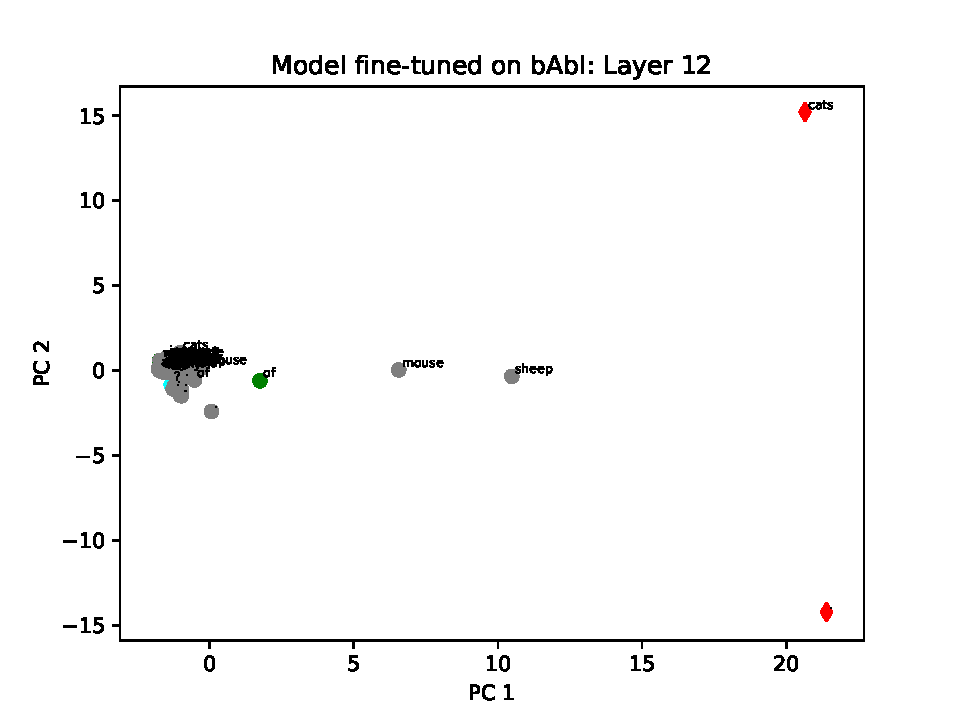
\includegraphics[scale=0.4]{../badges/reproduced/visualization/babi/model-fine-tuned-on-babi--layer-12.pdf}
		\end{tabular}
	\end{center}

	\subsection{Probing}
	Despite our best efforts, we were not able to get the Jiant Probing Suite set up and running and to reproduce the probing results from the paper. \\
	
	We initially tried to set up Jiant on Windows 10, but we had no success. Therefore we instead tried using a virtual machine running Linux (Ubuntu). Although we did have more success on Linux, we were still not able to get Jiant fully set up.
	
	Details about the error we received when we tried to run any of the experiments from the paper can be found below:\\
	
	We added the task we registered as the target task and set the input module to "bert-base-uncased". But when running the main.py script with this config file, we received the error "input length exceeds position embedding capacity, reduce max\_seq\_len" on the "Evaluating model on tasks" step. 
	
	The value used in the bert\_edgeprobe.conf is 512. We tried reducing the max\_seq\_len value in the config file to different values, as well as using the value from the defaults.conf file, but we always received this error.\\
	
	We discovered that this exact problem was discussed in multiple entries under the Issues tab on the jiant-v1-legacy GitHub repository. Sadly, none of these discussions offered an explanation or a solution to our problem. The majority of these discussions were automatically closed for the reason that the old version of Jiant will no longer be supported.
	
	With the documentation of the Jiant Probing Suite being rather sparsely, we were not able to find a solution to our problem or make any other progress on our own.\\
	
	We tried using the new version of the Jiant Probing Suite as well. But we had no luck with this version either.
	
	\section{Replicated}
	\subsection{Visualization}
	You can find our script that creates the visualizations for the hidden layers in the folder ./badges/replicated/visualization.\\
	
	The main script is visualization.py. The other script, visualization\_classes.py only holds the class definitions for the main script.
	
	To run our script, call the visualization.py. It accepts the following command line arguments:
	
	\begin{itemize}
		\item -sample: Path to the sample file
		\item -model: Path to the model file
		\item -type: Type of the model (optional, default: bert-base-uncased)
		\item -title: Title of the experiment (optional)
		\item -format: File format for the output (png,pdf,svg,jpg) (optional, default: png)
		\item --no-legend: If set, no legend will be added to the plots
	\end{itemize}

	The results will be saved to a subfolder of ./outputs, named like the experiment's title (set with -title`option). If the title of the experiment is not set, the current date and time will be used instead.\\

	
	You can find an example output from our script below. This is the plot our script generates for the squad sample from the paper.
	
	\begin{center}
		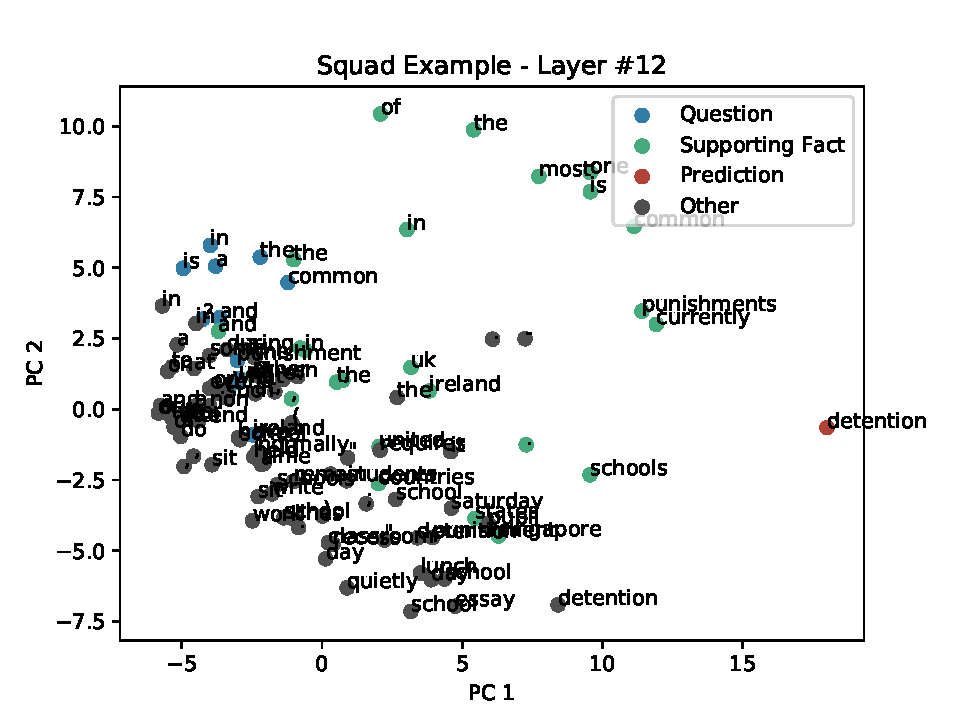
\includegraphics{../badges/replicated/visualization/output/squad-example/layer-12.pdf}
	\end{center}
	
	\section{New Code Variant}
	While experimenting with the visualization script from the explain-BERT-QA we discovered that it does not work well when the sample's context is longer than BERT's maximum length.
	
	...
	
\end{document}
